

\documentclass{article}%

\usepackage{amsmath}

\usepackage{graphicx}

\usepackage{amsfonts}%

\usepackage{amssymb}





\setlength{\topmargin}{-0.75in}

\setlength{\textheight}{9.25in}

\setlength{\oddsidemargin}{0.0in}

\setlength{\evensidemargin}{0.0in}

\setlength{\textwidth}{6.5in}

\def\labelenumi{\arabic{enumi}.}

\def\theenumi{\arabic{enumi}}

\def\labelenumii{(\alph{enumii})}

\def\theenumii{\alph{enumii}}

\def\p@enumii{\theenumi.}

\def\labelenumiii{\arabic{enumiii}.}

\def\theenumiii{\arabic{enumiii}}

\def\p@enumiii{(\theenumi)(\theenumii)}

\def\labelenumiv{\arabic{enumiv}.}

\def\theenumiv{\arabic{enumiv}}

\def\p@enumiv{\p@enumiii.\theenumiii}

\pagestyle{plain}

\setcounter{secnumdepth}{0}

\newtheorem{theorem}{Theorem}

\newtheorem{acknowledgement}[theorem]{Acknowledgement}

\newtheorem{algorithm}[theorem]{Algorithm}

\newtheorem{axiom}[theorem]{Axiom}

\newtheorem{case}[theorem]{Case}

\newtheorem{claim}[theorem]{Claim}

\newtheorem{conclusion}[theorem]{Conclusion}

\newtheorem{condition}[theorem]{Condition}

\newtheorem{conjecture}[theorem]{Conjecture}

\newtheorem{corollary}[theorem]{Corollary}

\newtheorem{criterion}[theorem]{Criterion}

\newtheorem{definition}[theorem]{Definition}

\newtheorem{example}[theorem]{Example}

\newtheorem{exercise}[theorem]{Exercise}

\newtheorem{lemma}[theorem]{Lemma}

\newtheorem{notation}[theorem]{Notation}

\newtheorem{problem}[theorem]{Problem}

\newtheorem{proposition}[theorem]{Proposition}

\newtheorem{remark}[theorem]{Remark}

\newtheorem{solution}[theorem]{Solution}

\newtheorem{summary}[theorem]{Summary}

\newenvironment{proof}[1][Proof]{\textbf{#1.} }{\ \rule{0.5em}{0.5em}}



\begin{document}



\begin{center}

\textbf{Homework 2}\bigskip

\end{center}





\noindent In problems 3. - 5., references such as III.2.7 refer to Problem 7 in Section 2 of Chapter III in Conway's book.\smallskip



\noindent If you use results from books including Conway's, please be explicit about what results you are using.






\begin{center}

\emph{Homework 2 is due on ICON by Midnight, February  11.}

\end{center} 

\medskip



\begin{enumerate}


\item Problem IV.1.5

\textbf{Sol.} By Proposition 1.3, 
$$
\begin{aligned}
V(\gamma) &= \int_{0}^{1}|\gamma'(t)|dt = \int_0^1 |\frac{1-i}{t^2}e^{\frac{-1+i}{t}}|dt = \int_{0}^{1} |\frac{1-i}{t^2}e^{-\frac{1}{t}}(\cos\frac{1}{t}+i\sin\frac{1}{t})|dt \\
&= \int_0^1\frac{e^{-\frac{1}{t}}}{t^2}\sqrt{(\cos\frac{1}{t}+\sin\frac{1}{t})^2+(\sin\frac{1}{t}-\cos\frac{1}{t})^2}dt = \int_0^1\sqrt{2}\frac{e^{-\frac{1}{t}}}{t^2}dt \\
&= \left.\sqrt{2}e^{-\frac{1}{t}}\right\arrowvert_{0}^{1} = \sqrt{2}e^{-1}.
\end{aligned}
$$
Hence $\gamma$ is rectifiable. The trace looks like the graph below:
\begin{figure}[!htb] \centering
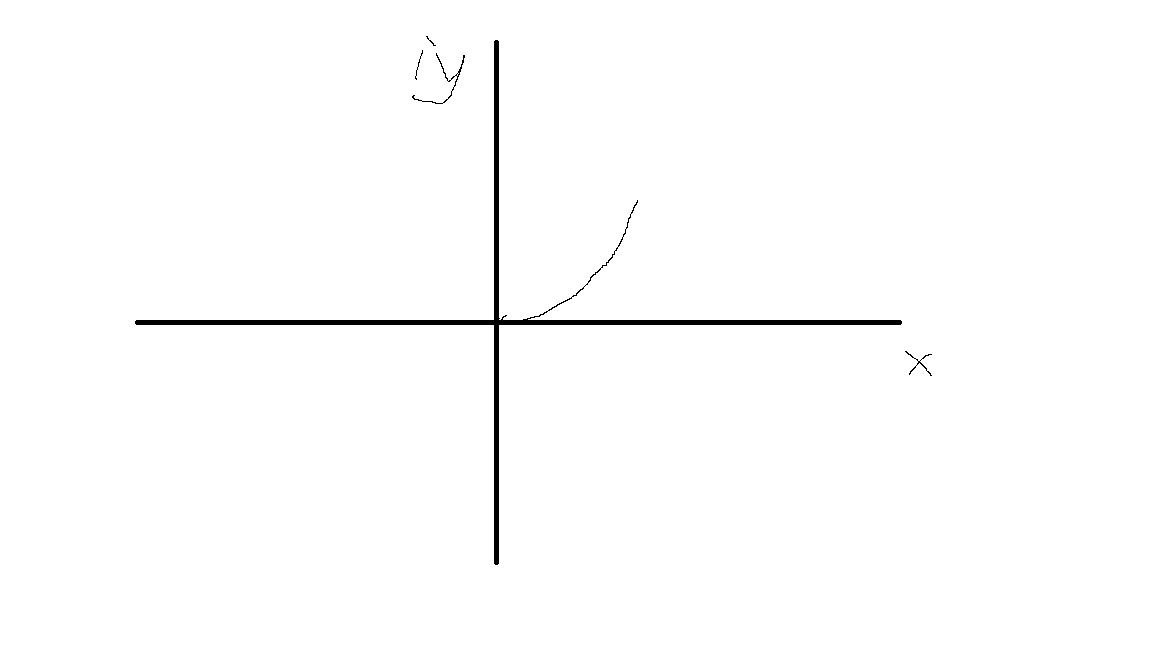
\includegraphics[width = 5cm]{prob1.jpg}
\end{figure}


\item Problem IV.1.9

\textbf{Sol.}
$$
\int_\gamma \frac{1}{z}dz = \int_{0}^{2\pi} e^{-int}ine^{int}dt = 2\pi in.
$$

\item Problem IV.1.12

\textbf{Sol.}
$$
I(r) = \int_{\gamma} \frac{e^{iz}}{z}dz = \int_{0}^{2\pi}\frac{e^{ire^{it}}}{re^{it}}ire^{it}dt = \int_{0}^{2\pi}ie^{ire^{it}}dt = \int_{0}^{2\pi}ie^{-r\sin t}(\cos(r\cos t)+i\sin(r\cos t))dt.
$$
Then 
$$
|I(r)| \le \int_{0}^{2\pi}|ie^{-r\sin t}(\cos(r\cos t)+i\sin(r\cos t))|dt = \int_0^{2\pi}e^{-r\sin t}dt = \int_{0}^{\pi}+\int_{\pi}^{2\pi}e^{-r\sin t}dt.
$$
Pick an arbitrary $\epsilon > 0$, the first term
$$
\int_{0}^{\pi}e^{-r\sin t}dt = \int_0^\epsilon + \int_\epsilon^{\pi-\epsilon} + \int_{\pi-\epsilon}^{\pi}e^{-r\sin t}dt \le 2\epsilon + (\pi-2\epsilon)e^{-r\sin\epsilon}.
$$
Then when $r \to \infty$,
$$
\int_{0}^{\pi}e^{-r\sin t}dt \le 2\epsilon.
$$
By the arbitrariness of $\epsilon$, $\int_{0}^{\pi}e^{-r\sin t}dt \to 0$ when $r\to \infty$. It is the same for the second term $\int_{\pi}^{2\pi} $. Hence $\lim\limits_{r\to\infty}I(r) = 0 $.

\item Problem IV.1.13

\textbf{Sol (a).} 
$$
\int_{\gamma}z^{-\frac{1}{2}}dz = \left.\int_{0}^{\pi}e^{-\frac{1}{2}it}ie^{it}dt = 2e^{\frac{1}{2}it}\right\arrowvert_{0}^{\pi} = 2i-2.
$$
\textbf{(b).}
$$
\int_{\gamma}z^{-\frac{1}{2}}dz = \left.\int_{2\pi}^{\pi}e^{-\frac{1}{2}it}ie^{it}dt = 2e^{\frac{1}{2}it}\right\arrowvert_{2\pi}^{\pi} = 2i+2.
$$

\item Problem IV.1.14

\textbf{Proof.} First, assume $\varphi$ is one-one. Then if $\varphi$ is not strictly increasing, suppose there exists $x < y \in [a, b]$, s.t. $\varphi(x) \ge \varphi(y)$. If $\varphi(x) = \varphi(y)$, it contradicts with that $\varphi$ is one-one. So $\varphi(x) > \varphi(y)$. Since $\varphi(x) > c$ (otherwise $\varphi(y) < c$ contradicts with $\varphi([a, b]) \ge c$), by continuity of $\varphi$, $\exists z \in [a, x]$, s.t. $\varphi(z) = \varphi(y)$, which makes a contradiction. Thus $\varphi$ is strictly increasing.

Now assume $\varphi$ is strictly increasing, then $\varphi$ is an injection. Besides, for each $y\in [c, d]$, by continuity of $\varphi$, there is a $x\in[a, b]$, s.t. $\varphi(x) = y$. Hence $\varphi$ is a bijection.

\item Problem IV.1.20

\textbf{Sol.} 
$$
\int_{\gamma}\frac{1}{z^2-1}dz = \int_{0}^{2\pi}\frac{1}{(e^{it}+1)^2-1}ie^{it}dt = \left.\int_{0}^{2\pi}\frac{i}{2+e^{it}}dt = \frac{1}{2}i(t+i\ln(2+e^{it}))\right\arrowvert_{0}^{2\pi} = \pi i
$$

\item Problem IV.2.1

\textbf{Proof.} We need to show that $g$ is continuous at each $t_0\in[c, d] $. In fact, $\forall \epsilon > 0$, since $\varphi$ is continuous, $\exists \delta > 0$, when $|t_1-t_0| < \delta $, we have $|\varphi(s, t_1)-\varphi(s, t_0)| < \frac{\epsilon}{b-a}$. Thus when $|t_1-t_0| < \delta $,
$$
|g(t_1)-g(t_0)| \le \int_{a}^{b}|\varphi(s, t_1)-\varphi(s, t_2)|ds < \int_{a}^{b}\frac{\epsilon}{b-a}ds = \epsilon.
$$
Hence $g$ is continuous at $t_0 $.

\item Problem IV.2.2  (Please note.  This problem will be used a number of places in the theory we will develop.)

\textbf{Proof.} 

\item Problem IV.2.3

\end{enumerate}

\end{document}

